\documentclass{standalone}
\usepackage{tikz}
\usetikzlibrary{patterns, positioning}
\usepackage[sfdefault]{ClearSans} %% option 'sfdefault' activates Clear Sans as the default text font
\usepackage[T1]{fontenc}

\begin{document}
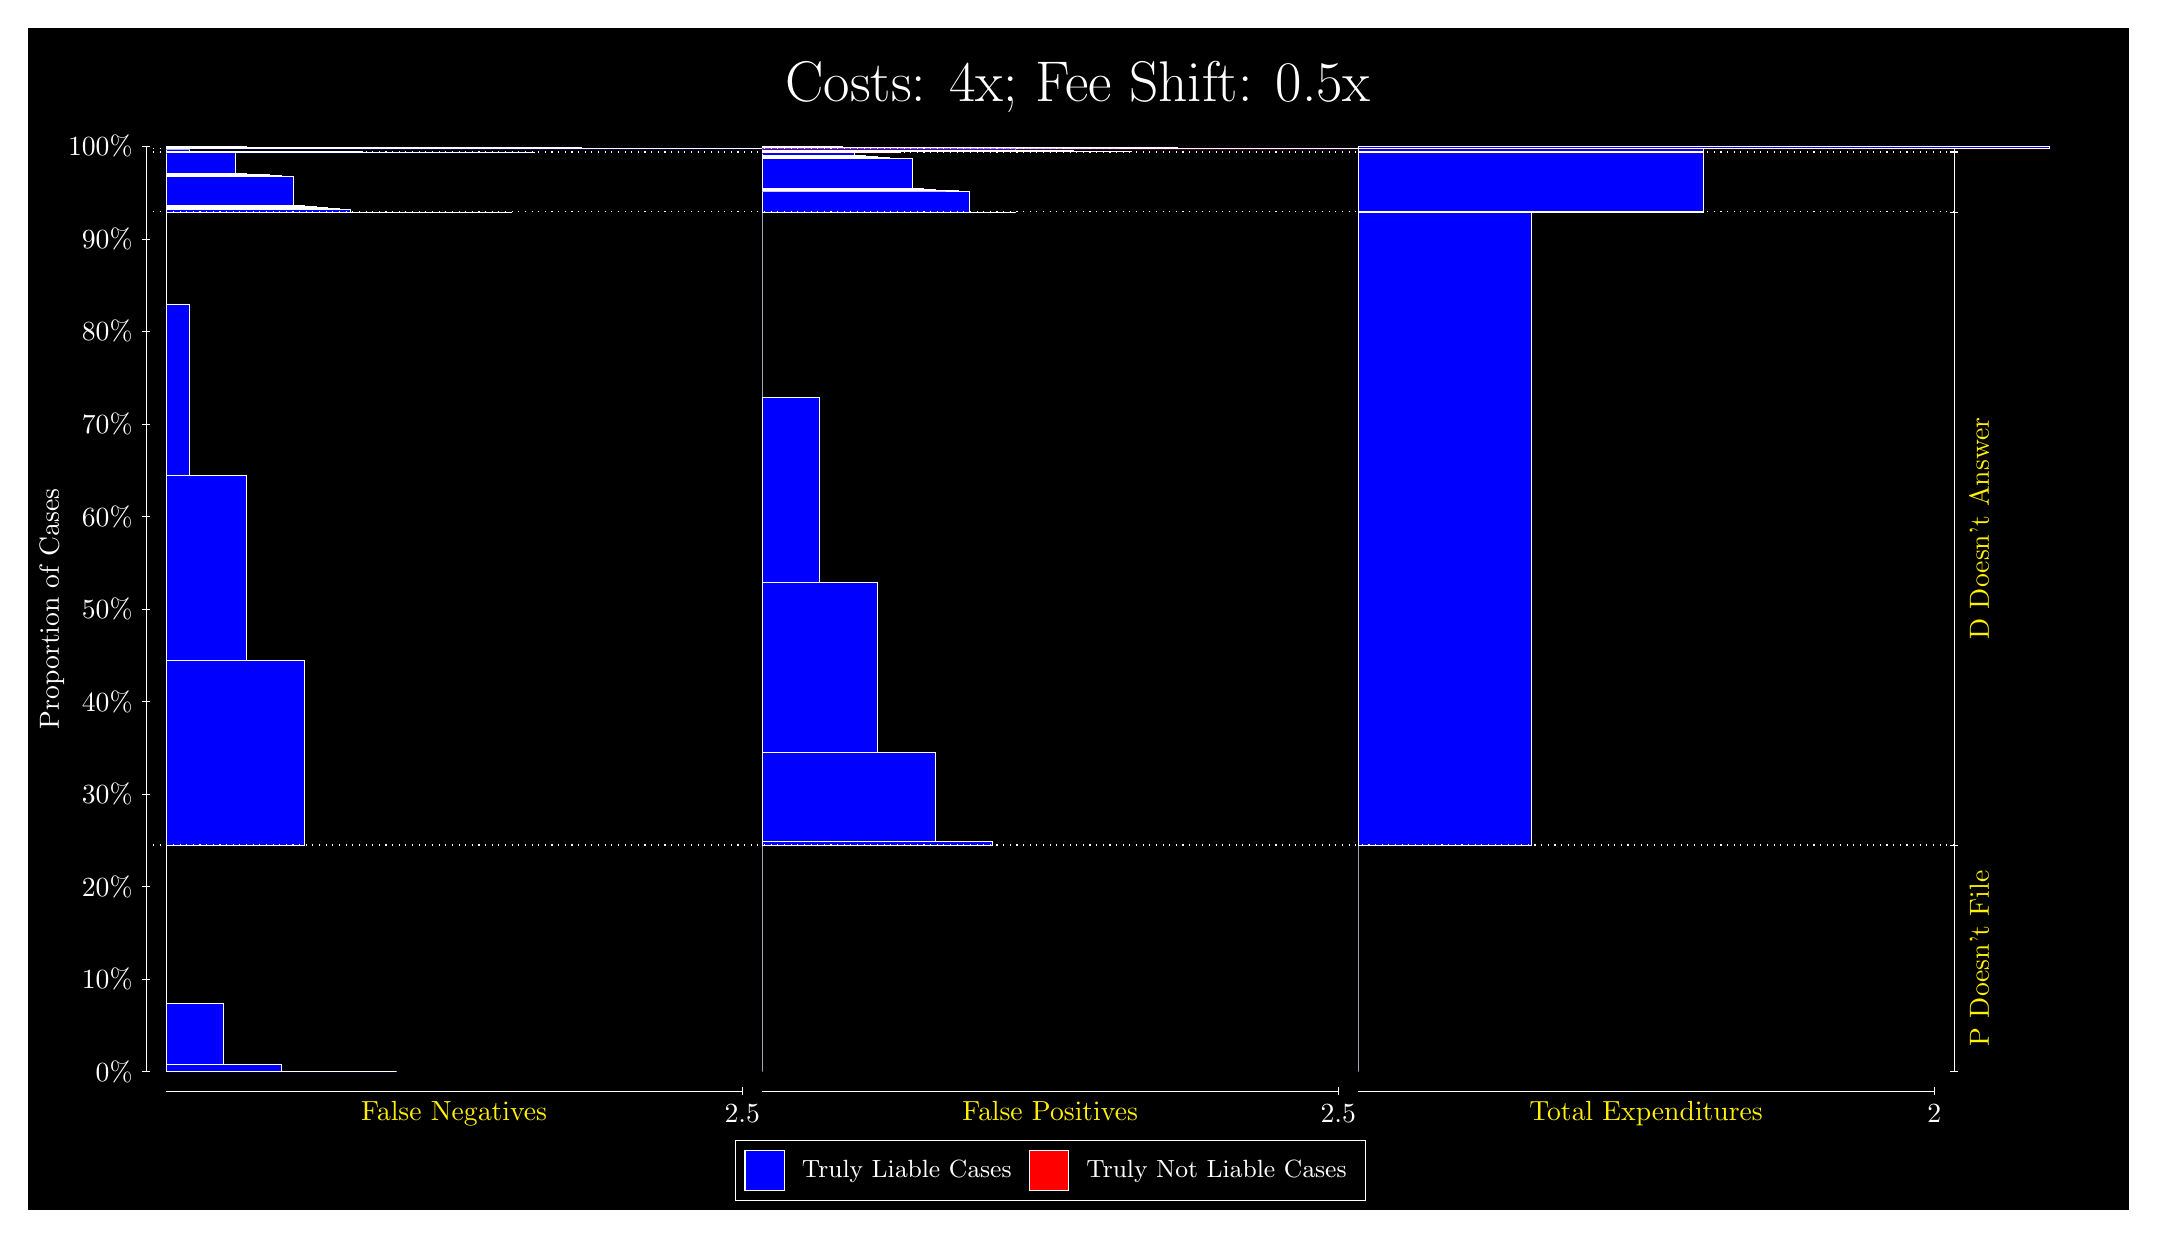
\begin{tikzpicture}
\draw[fill=black] (0,0) rectangle (26.667,15);
\draw[text=white] (0,13.5) rectangle (26.667,15) node[midway] {\huge Costs: 4x; Fee Shift: 0.5x};
\draw[white, very thin] (1.5,1.75) -- (1.5,13.5);
\node[rotate=90, text=white, anchor=center] at (0.3, 7.625) {Proportion of Cases};
\draw[white, very thin] (1.45,1.75) -- (1.55,1.75);
\node[text=white, anchor=east] at (1.45, 1.75) {0\%};
\draw[white, very thin] (1.45,2.925) -- (1.55,2.925);
\node[text=white, anchor=east] at (1.45, 2.925) {10\%};
\draw[white, very thin] (1.45,4.1) -- (1.55,4.1);
\node[text=white, anchor=east] at (1.45, 4.1) {20\%};
\draw[white, very thin] (1.45,5.275) -- (1.55,5.275);
\node[text=white, anchor=east] at (1.45, 5.275) {30\%};
\draw[white, very thin] (1.45,6.45) -- (1.55,6.45);
\node[text=white, anchor=east] at (1.45, 6.45) {40\%};
\draw[white, very thin] (1.45,7.625) -- (1.55,7.625);
\node[text=white, anchor=east] at (1.45, 7.625) {50\%};
\draw[white, very thin] (1.45,8.8) -- (1.55,8.8);
\node[text=white, anchor=east] at (1.45, 8.8) {60\%};
\draw[white, very thin] (1.45,9.975) -- (1.55,9.975);
\node[text=white, anchor=east] at (1.45, 9.975) {70\%};
\draw[white, very thin] (1.45,11.15) -- (1.55,11.15);
\node[text=white, anchor=east] at (1.45, 11.15) {80\%};
\draw[white, very thin] (1.45,12.325) -- (1.55,12.325);
\node[text=white, anchor=east] at (1.45, 12.325) {90\%};
\draw[white, very thin] (1.45,13.5) -- (1.55,13.5);
\node[text=white, anchor=east] at (1.45, 13.5) {100\%};

\draw[white, very thin] (24.457,1.75) -- (24.457,13.5);
\draw[white, very thin] (24.407,1.75) -- (24.507,1.75);
\node[anchor=west] at (24.407, 1.75) {};
\draw[white, very thin] (24.407,4.6267) -- (24.507,4.6267);
\node[anchor=west] at (24.407, 4.6267) {};
\draw[white, very thin] (24.407,12.667) -- (24.507,12.667);
\node[anchor=west] at (24.407, 12.667) {};
\draw[white, very thin] (24.407,13.421) -- (24.507,13.421);
\node[anchor=west] at (24.407, 13.421) {};
\draw[white, very thin] (24.407,13.439) -- (24.507,13.439);
\node[anchor=west] at (24.407, 13.439) {};
\draw[white, very thin] (24.407,13.472) -- (24.507,13.472);
\node[anchor=west] at (24.407, 13.472) {};
\draw[white, very thin] (24.407,13.5) -- (24.507,13.5);
\node[anchor=west] at (24.407, 13.5) {};

\draw[white, very thin, fill=blue] (1.75,1.75) rectangle (4.6775,1.75);
\draw[white, very thin, fill=blue] (1.75,1.75) rectangle (3.9457,1.7508);
\draw[white, very thin, fill=blue] (1.75,1.7508) rectangle (3.2138,1.8451);
\draw[white, very thin, fill=blue] (1.75,1.8451) rectangle (2.4819,2.6115);
\draw[white, very thin, fill=red] (1.75,2.6115) rectangle (1.75,2.6115);
\draw[white, very thin, fill=blue] (1.75,2.6115) rectangle (1.75,4.6267);
\draw[white, very thin, fill=blue] (1.75,4.6267) rectangle (3.5065,6.9767);
\draw[white, very thin, fill=blue] (1.75,6.9767) rectangle (2.7746,9.3251);
\draw[white, very thin, fill=blue] (1.75,9.3251) rectangle (2.0428,11.493);
\draw[white, very thin, fill=red] (1.75,11.493) rectangle (1.75,11.493);
\draw[white, very thin, fill=blue] (1.75,11.493) rectangle (1.75,12.667);
\draw[white, very thin, fill=blue] (1.75,12.667) rectangle (6.1413,12.667);
\draw[white, very thin, fill=blue] (1.75,12.667) rectangle (5.8486,12.667);
\draw[white, very thin, fill=blue] (1.75,12.667) rectangle (5.5558,12.667);
\draw[white, very thin, fill=blue] (1.75,12.667) rectangle (5.4094,12.667);
\draw[white, very thin, fill=blue] (1.75,12.667) rectangle (5.2631,12.667);
\draw[white, very thin, fill=blue] (1.75,12.667) rectangle (5.1167,12.667);
\draw[white, very thin, fill=blue] (1.75,12.667) rectangle (4.9703,12.667);
\draw[white, very thin, fill=blue] (1.75,12.667) rectangle (4.8239,12.667);
\draw[white, very thin, fill=blue] (1.75,12.667) rectangle (4.6775,12.667);
\draw[white, very thin, fill=blue] (1.75,12.667) rectangle (4.5312,12.667);
\draw[white, very thin, fill=blue] (1.75,12.667) rectangle (4.3848,12.668);
\draw[white, very thin, fill=blue] (1.75,12.668) rectangle (4.2384,12.668);
\draw[white, very thin, fill=blue] (1.75,12.668) rectangle (4.092,12.705);
\draw[white, very thin, fill=blue] (1.75,12.705) rectangle (3.9457,12.716);
\draw[white, very thin, fill=blue] (1.75,12.716) rectangle (3.7993,12.731);
\draw[white, very thin, fill=blue] (1.75,12.731) rectangle (3.6529,12.738);
\draw[white, very thin, fill=blue] (1.75,12.738) rectangle (3.5065,12.746);
\draw[white, very thin, fill=blue] (1.75,12.746) rectangle (3.3602,13.121);
\draw[white, very thin, fill=blue] (1.75,13.121) rectangle (3.2138,13.135);
\draw[white, very thin, fill=blue] (1.75,13.135) rectangle (3.0674,13.15);
\draw[white, very thin, fill=blue] (1.75,13.15) rectangle (2.921,13.151);
\draw[white, very thin, fill=blue] (1.75,13.151) rectangle (2.7746,13.155);
\draw[white, very thin, fill=blue] (1.75,13.155) rectangle (2.6283,13.421);
\draw[white, very thin, fill=blue] (1.75,13.421) rectangle (2.3355,13.421);
\draw[white, very thin, fill=blue] (1.75,13.421) rectangle (2.0428,13.421);
\draw[white, very thin, fill=red] (1.75,13.421) rectangle (1.75,13.421);
\draw[white, very thin, fill=blue] (1.75,13.421) rectangle (6.4341,13.421);
\draw[white, very thin, fill=blue] (1.75,13.421) rectangle (5.7022,13.421);
\draw[white, very thin, fill=blue] (1.75,13.421) rectangle (4.9703,13.424);
\draw[white, very thin, fill=blue] (1.75,13.424) rectangle (4.2384,13.439);
\draw[white, very thin, fill=blue] (1.75,13.439) rectangle (3.5065,13.439);
\draw[white, very thin, fill=red] (1.75,13.439) rectangle (1.75,13.439);
\draw[white, very thin, fill=blue] (1.75,13.439) rectangle (3.5065,13.439);
\draw[white, very thin, fill=blue] (1.75,13.439) rectangle (2.7746,13.44);
\draw[white, very thin, fill=blue] (1.75,13.44) rectangle (2.0428,13.46);
\draw[white, very thin, fill=red] (1.75,13.46) rectangle (1.75,13.46);
\draw[white, very thin, fill=blue] (1.75,13.46) rectangle (1.75,13.472);
\draw[white, very thin, fill=blue] (1.75,13.472) rectangle (9.9471,13.472);
\draw[white, very thin, fill=blue] (1.75,13.472) rectangle (9.2152,13.472);
\draw[white, very thin, fill=blue] (1.75,13.472) rectangle (8.4834,13.472);
\draw[white, very thin, fill=blue] (1.75,13.472) rectangle (7.7515,13.478);
\draw[white, very thin, fill=blue] (1.75,13.478) rectangle (7.0196,13.488);
\draw[white, very thin, fill=blue] (1.75,13.488) rectangle (6.2877,13.488);
\draw[white, very thin, fill=blue] (1.75,13.488) rectangle (5.7022,13.488);
\draw[white, very thin, fill=blue] (1.75,13.488) rectangle (5.5558,13.488);
\draw[white, very thin, fill=blue] (1.75,13.488) rectangle (4.9703,13.488);
\draw[white, very thin, fill=blue] (1.75,13.488) rectangle (4.2384,13.488);
\draw[white, very thin, fill=blue] (1.75,13.488) rectangle (3.5065,13.493);
\draw[white, very thin, fill=blue] (1.75,13.493) rectangle (2.7746,13.499);
\draw[white, very thin, fill=blue] (1.75,13.499) rectangle (2.0428,13.5);
\draw[white, very thin, fill=red] (1.75,13.5) rectangle (1.75,13.5);
\draw[white, very thin, fill=blue] (1.75,13.5) rectangle (1.75,13.5);
\draw[white, very thin, fill=red] (9.3189,1.75) rectangle (9.3189,1.75);
\draw[white, very thin, fill=blue] (9.3189,1.75) rectangle (9.3189,4.6267);
\draw[white, very thin, fill=red] (9.3189,4.6267) rectangle (12.246,4.6267);
\draw[white, very thin, fill=blue] (9.3189,4.6267) rectangle (12.246,4.6785);
\draw[white, very thin, fill=blue] (9.3189,4.6785) rectangle (11.515,5.8008);
\draw[white, very thin, fill=blue] (9.3189,5.8008) rectangle (10.783,7.9687);
\draw[white, very thin, fill=blue] (9.3189,7.9687) rectangle (10.051,10.317);
\draw[white, very thin, fill=blue] (9.3189,10.317) rectangle (9.3189,12.667);
\draw[white, very thin, fill=red] (9.3189,12.667) rectangle (12.539,12.667);
\draw[white, very thin, fill=blue] (9.3189,12.667) rectangle (12.539,12.667);
\draw[white, very thin, fill=red] (9.3189,12.667) rectangle (12.246,12.667);
\draw[white, very thin, fill=blue] (9.3189,12.667) rectangle (12.246,12.667);
\draw[white, very thin, fill=red] (9.3189,12.667) rectangle (11.954,12.667);
\draw[white, very thin, fill=blue] (9.3189,12.667) rectangle (11.954,12.934);
\draw[white, very thin, fill=blue] (9.3189,12.934) rectangle (11.807,12.938);
\draw[white, very thin, fill=red] (9.3189,12.938) rectangle (11.661,12.938);
\draw[white, very thin, fill=blue] (9.3189,12.938) rectangle (11.661,12.938);
\draw[white, very thin, fill=blue] (9.3189,12.938) rectangle (11.515,12.953);
\draw[white, very thin, fill=red] (9.3189,12.953) rectangle (11.368,12.953);
\draw[white, very thin, fill=blue] (9.3189,12.953) rectangle (11.368,12.967);
\draw[white, very thin, fill=blue] (9.3189,12.967) rectangle (11.222,13.342);
\draw[white, very thin, fill=blue] (9.3189,13.342) rectangle (11.075,13.35);
\draw[white, very thin, fill=blue] (9.3189,13.35) rectangle (10.929,13.358);
\draw[white, very thin, fill=blue] (9.3189,13.358) rectangle (10.783,13.373);
\draw[white, very thin, fill=blue] (9.3189,13.373) rectangle (10.636,13.384);
\draw[white, very thin, fill=blue] (9.3189,13.384) rectangle (10.49,13.421);
\draw[white, very thin, fill=blue] (9.3189,13.421) rectangle (10.344,13.421);
\draw[white, very thin, fill=blue] (9.3189,13.421) rectangle (10.197,13.421);
\draw[white, very thin, fill=blue] (9.3189,13.421) rectangle (10.051,13.421);
\draw[white, very thin, fill=blue] (9.3189,13.421) rectangle (9.9044,13.421);
\draw[white, very thin, fill=blue] (9.3189,13.421) rectangle (9.758,13.421);
\draw[white, very thin, fill=blue] (9.3189,13.421) rectangle (9.6116,13.421);
\draw[white, very thin, fill=blue] (9.3189,13.421) rectangle (9.4652,13.421);
\draw[white, very thin, fill=blue] (9.3189,13.421) rectangle (9.3189,13.421);
\draw[white, very thin, fill=red] (9.3189,13.421) rectangle (11.075,13.421);
\draw[white, very thin, fill=blue] (9.3189,13.421) rectangle (11.075,13.422);
\draw[white, very thin, fill=blue] (9.3189,13.422) rectangle (10.344,13.437);
\draw[white, very thin, fill=blue] (9.3189,13.437) rectangle (9.6116,13.439);
\draw[white, very thin, fill=blue] (9.3189,13.439) rectangle (9.3189,13.439);
\draw[white, very thin, fill=red] (9.3189,13.439) rectangle (14.003,13.439);
\draw[white, very thin, fill=blue] (9.3189,13.439) rectangle (14.003,13.44);
\draw[white, very thin, fill=blue] (9.3189,13.44) rectangle (13.271,13.452);
\draw[white, very thin, fill=blue] (9.3189,13.452) rectangle (12.539,13.472);
\draw[white, very thin, fill=blue] (9.3189,13.472) rectangle (11.807,13.472);
\draw[white, very thin, fill=blue] (9.3189,13.472) rectangle (11.075,13.472);
\draw[white, very thin, fill=red] (9.3189,13.472) rectangle (17.516,13.472);
\draw[white, very thin, fill=blue] (9.3189,13.472) rectangle (17.516,13.472);
\draw[white, very thin, fill=red] (9.3189,13.472) rectangle (16.784,13.472);
\draw[white, very thin, fill=blue] (9.3189,13.472) rectangle (16.784,13.472);
\draw[white, very thin, fill=red] (9.3189,13.472) rectangle (16.052,13.472);
\draw[white, very thin, fill=blue] (9.3189,13.472) rectangle (16.052,13.473);
\draw[white, very thin, fill=red] (9.3189,13.473) rectangle (15.32,13.473);
\draw[white, very thin, fill=blue] (9.3189,13.473) rectangle (15.32,13.479);
\draw[white, very thin, fill=blue] (9.3189,13.479) rectangle (14.588,13.484);
\draw[white, very thin, fill=blue] (9.3189,13.484) rectangle (13.857,13.484);
\draw[white, very thin, fill=blue] (9.3189,13.484) rectangle (13.125,13.484);
\draw[white, very thin, fill=red] (9.3189,13.484) rectangle (12.539,13.484);
\draw[white, very thin, fill=blue] (9.3189,13.484) rectangle (12.539,13.484);
\draw[white, very thin, fill=blue] (9.3189,13.484) rectangle (12.393,13.484);
\draw[white, very thin, fill=blue] (9.3189,13.484) rectangle (11.807,13.484);
\draw[white, very thin, fill=red] (9.3189,13.484) rectangle (11.807,13.484);
\draw[white, very thin, fill=blue] (9.3189,13.484) rectangle (11.807,13.484);
\draw[white, very thin, fill=blue] (9.3189,13.484) rectangle (11.075,13.484);
\draw[white, very thin, fill=red] (9.3189,13.484) rectangle (11.075,13.484);
\draw[white, very thin, fill=blue] (9.3189,13.484) rectangle (11.075,13.494);
\draw[white, very thin, fill=blue] (9.3189,13.494) rectangle (10.344,13.494);
\draw[white, very thin, fill=blue] (9.3189,13.494) rectangle (10.344,13.5);
\draw[white, very thin, fill=blue] (9.3189,13.5) rectangle (9.6116,13.5);
\draw[white, very thin, fill=blue] (9.3189,13.5) rectangle (9.6116,13.5);
\draw[white, very thin, fill=blue] (9.3189,13.5) rectangle (9.3189,13.5);
\draw[white, very thin, fill=red] (16.888,1.75) rectangle (16.888,1.75);
\draw[white, very thin, fill=blue] (16.888,1.75) rectangle (16.888,4.6267);
\draw[white, very thin, fill=red] (16.888,4.6267) rectangle (19.083,4.6267);
\draw[white, very thin, fill=blue] (16.888,4.6267) rectangle (19.083,12.667);
\draw[white, very thin, fill=red] (16.888,12.667) rectangle (21.279,12.667);
\draw[white, very thin, fill=blue] (16.888,12.667) rectangle (21.279,12.679);
\draw[white, very thin, fill=red] (16.888,12.679) rectangle (21.279,12.679);
\draw[white, very thin, fill=blue] (16.888,12.679) rectangle (21.279,13.421);
\draw[white, very thin, fill=red] (16.888,13.421) rectangle (21.279,13.421);
\draw[white, very thin, fill=blue] (16.888,13.421) rectangle (21.279,13.439);
\draw[white, very thin, fill=red] (16.888,13.439) rectangle (21.279,13.439);
\draw[white, very thin, fill=blue] (16.888,13.439) rectangle (21.279,13.472);
\draw[white, very thin, fill=red] (16.888,13.472) rectangle (25.67,13.472);
\draw[white, very thin, fill=blue] (16.888,13.472) rectangle (25.67,13.5);
\draw[white, dotted] (1.5,4.6267) -- (24.457,4.6267);
\draw[white, dotted] (1.5,12.667) -- (24.457,12.667);
\draw[white, dotted] (1.5,13.421) -- (24.457,13.421);
\draw[white, dotted] (1.5,13.439) -- (24.457,13.439);
\draw[white, dotted] (1.5,13.472) -- (24.457,13.472);
\draw[white, very thin] (1.75,1.5) -- (9.0689,1.5);
\node[text=yellow, anchor=north] at (5.4094, 1.5) {False Negatives};
\draw[white, very thin] (9.0689,1.45) -- (9.0689,1.55);
\node[text=white, anchor=north] at (9.0689, 1.45) {2.5};

\draw[white, very thin] (9.3189,1.5) -- (16.638,1.5);
\node[text=yellow, anchor=north] at (12.978, 1.5) {False Positives};
\draw[white, very thin] (16.638,1.45) -- (16.638,1.55);
\node[text=white, anchor=north] at (16.638, 1.45) {2.5};

\draw[white, very thin] (16.888,1.5) -- (24.207,1.5);
\node[text=yellow, anchor=north] at (20.547, 1.5) {Total Expenditures};
\draw[white, very thin] (24.207,1.45) -- (24.207,1.55);
\node[text=white, anchor=north] at (24.207, 1.45) {2};

\node[text=yellow, centered, rotate=90] at (24.777, 3.1884) {P Doesn't File};
\node[text=yellow, centered, rotate=90] at (24.777, 8.6469) {D Doesn't Answer};





\draw (12.978300999999998,1.5) node[draw=none] (baseCoordinate) {};
\begin{scope}[align=center]
        \matrix[scale=0.5, draw=white, below=0.5cm of baseCoordinate, nodes={draw}, column sep=0.1cm]{
            \node[rectangle, draw, minimum width=0.5cm, minimum height=0.5cm, fill=blue] {}; &
            \node[draw=none, font=\small, text=white] (B) {Truly Liable Cases}; &
            \node[rectangle, draw, minimum width=0.5cm, minimum height=0.5cm, fill=red] {}; &
            \node[draw=none, font=\small, text=white] (B) {Truly Not Liable Cases}; \\
            };
\end{scope}

\end{tikzpicture}
\end{document}